%%%%%%%%%%%%%%%%%%%%%%%%%%%%%%%%%%%%%%%%%%%%%%%%%%%%%%%%%%%%%%%%%%%%%%%%%%%%%%%%%%%%%%%%
\chapter{Chiral Spin Liquids on the Hypernonagon Lattice (9,3)a}
\label{chapter:HypernonagonLattice}
%%%%%%%%%%%%%%%%%%%%%%%%%%%%%%%%%%%%%%%%%%%%%%%%%%%%%%%%%%%%%%%%%%%%%%%%%%%%%%%%%%%%%%%%
%
%
\footnote{This chapter discusses work which is to be reported in Reference~\cite{MischenkoPRB2019}. P~.A. Mishchenko and Y. Kato are responsible for determining the ground state flux configurations, while the author of this thesis performed the analysis of the fermionic excitations.}The previous chapter introduced a number of three-dimensional, tricoordinated lattices and analyzed the physics of the Kitaev model defined on these lattices.
The end result of this analysis was to provide a method for classifying the stable, gapless quantum spin liquids on these lattices making use of an object called the projective symmetry group.
The detailed analysis of the Kitaev model on these lattices served to illustrate the power of this method for explaining the ground state properties of the gapless quantum spin liquid phases as well as to provide an understanding of the stability of the resulting low-energy features.

In this analysis, two lattices stood out due to the fact that their ground state flux configurations could not be readily inferred from Lieb's theorem.
The first of these was lattice (8,3)c.
Here, the complication arises from a frustration of the gauge field due to flux volume constraints.
As mentioned in the previous chapter, the Kitaev model on this lattice has subsequently been investigated in Reference~\cite{EschmannPRL2019} where it was shown that, although the ground state flux configuration is more complicated than that used in the analysis of Chapter~\ref{chapter:ClassificationOfKSL}, the general statements made therein about the properties of the gapless fermionic excitations remain accurate.
The other such lattice, lattice (9,3)a, is the subject of the present chapter.

The remainder of this chapter is structured as follows.
Section~\ref{section:chapter06_Lattice} provides detailed information on a deformed version of lattice (9,3)a that is used in the analysis presented in this chapter.
Section~\ref{section:chapter06_Fluxes} discusses the \ZZ~fluxes throughout the ground state phase diagram as well as information about the quantum Monte Carlo methods used by collaborators of the present author to investigate them.
In all cases, the ground state flux configuration breaks time-reversal symmetry spontaneously due to the non-bipartiteness of the underlying lattice, resulting in a \textit{chiral} spin liquid ground state.
Section~\ref{section:chapter06_GaplessSpinLiquids} makes use of this flux information to solve for the ground state phase diagram of the fermionic quasiparticles and provides a detailed discussion of the gapless portions of this phase diagram.
In some cases, the analysis follows directly from the classification scheme presented in the previous chapter, however, in one case the results go beyond this classification showing a possibility which was previously overlooked.
Finally, Section~\ref{section:chapter06_Conclusion} provides a brief recapitulation of the results.


%
%
%%%%%%%%%%%%%%%%%%%%%%%%%%%%%%%%%%%%%%%%%%%%%%%%%%%%%%%%%%%%%%%%%%%%%%%%%%%%%%%%%%%%%%%%
\section{Lattice information}
\label{section:chapter06_Lattice}
%%%%%%%%%%%%%%%%%%%%%%%%%%%%%%%%%%%%%%%%%%%%%%%%%%%%%%%%%%%%%%%%%%%%%%%%%%%%%%%%%%%%%%%%
%
%
As mentioned in Section~\ref{section:chapter05_9_3a}, it is possible to define an equivalent, but deformed version of lattice (9,3)a in terms of honeycomb layers joined by mid-bond sites.
The concrete choice of elementary unit cell for this deformed lattice has twelve sites with positions given by
%
\begin{equation}
	\begin{matrix*}[l]
		\br_1 = \left(0, 0, 0\right) &
		\br_2 = \left(-\frac{1}{4\sqrt{3}}, \frac{1}{4}, 0\right) &
		\br_3 = \left(-\frac{1}{2\sqrt{3}}, \frac{1}{2}, 0\right) \\
		&\\
		\br_4 = \left(-\frac{1}{\sqrt{3}}, \frac{1}{2}, 0\right) &
		\br_5 = \left(-\frac{\sqrt{3}}{2}, \frac{1}{2}, 0\right) &
		\br_6 = \left(-\frac{7}{4\sqrt{3}}, \frac{1}{4}, 0\right) \\
		&\\
		\br_7 = \left(-\frac{2}{\sqrt{3}}, 0, 0\right) &
		\br_8 = \left(-\frac{7}{4\sqrt{3}}, -\frac{1}{4}, 0\right) &
		\br_9 = \left(-\frac{\sqrt{3}}{2}, -\frac{1}{2}, 0\right) \\
		&\\
		\br_{10} = \left(-\frac{1}{\sqrt{3}}, -\frac{1}{2}, 0\right) &
		\br_{11} = \left(-\frac{1}{2\sqrt{3}}, -\frac{1}{2}, 0\right) &
		\br_{12} = \left(-\frac{1}{4\sqrt{3}}, -\frac{1}{4}, 0\right).
	\end{matrix*}
\end{equation}
%
The lattice vectors are chosen to be
%
\begin{equation}
	\begin{matrix*}[l]
		\ba_1 = \left(-\frac{\sqrt{3}}{2}, \frac{1}{2}, \frac{1}{\sqrt{3}}\right) \qquad
		\ba_2 = \left(0, -1, \frac{1}{\sqrt{3}}\right) \qquad
		\ba_3 = \left(\frac{\sqrt{3}}{2}, \frac{1}{2}, \frac{1}{\sqrt{3}}\right)
	\end{matrix*}
\end{equation}
%
with corresponding reciprocal lattice vectors
%
\begin{equation}
	\begin{matrix*}[l]
		\bq_1 = \left(-\frac{2\pi}{\sqrt{3}}, \frac{2\pi}{3}, \frac{2\pi}{\sqrt{3}}\right) \qquad
		\bq_2 = \left(0, -\frac{4\pi}{3}, \frac{2\pi}{\sqrt{3}}\right) \qquad
		\bq_3 = \left(\frac{2\pi}{\sqrt{3}}, \frac{2\pi}{3}, \frac{2\pi}{\sqrt{3}}\right).
	\end{matrix*}
\end{equation}
%

The unit cell and translation vectors are illustrated in Figure~\ref{fig:chapter06_9_3aPanel}~(a).
The bonds in the figure are colored red, green and blue to indicate the assignment of $x$-, $y$- and $z$-type bonds, respectively.
Up to permutation of the bond types, this assignment is unique when preserving all lattice symmetries.
All $x$- and $y$-bonds are related by a combination of $C_3$ and mirror symmetries.
There are two distinct sets of $z$-bonds which are not related by lattice symmetries, however, all bonds of a given set may be mapped onto each other by a $C_3$ symmetry.
The symmetry between $x$- and $y$-bonds is reflected in the ground state phase diagrams of Figures~\ref{fig:chapter06_9_3aPanel}~(b) and (c).
%
\begin{figure}[tb]
	\centering
	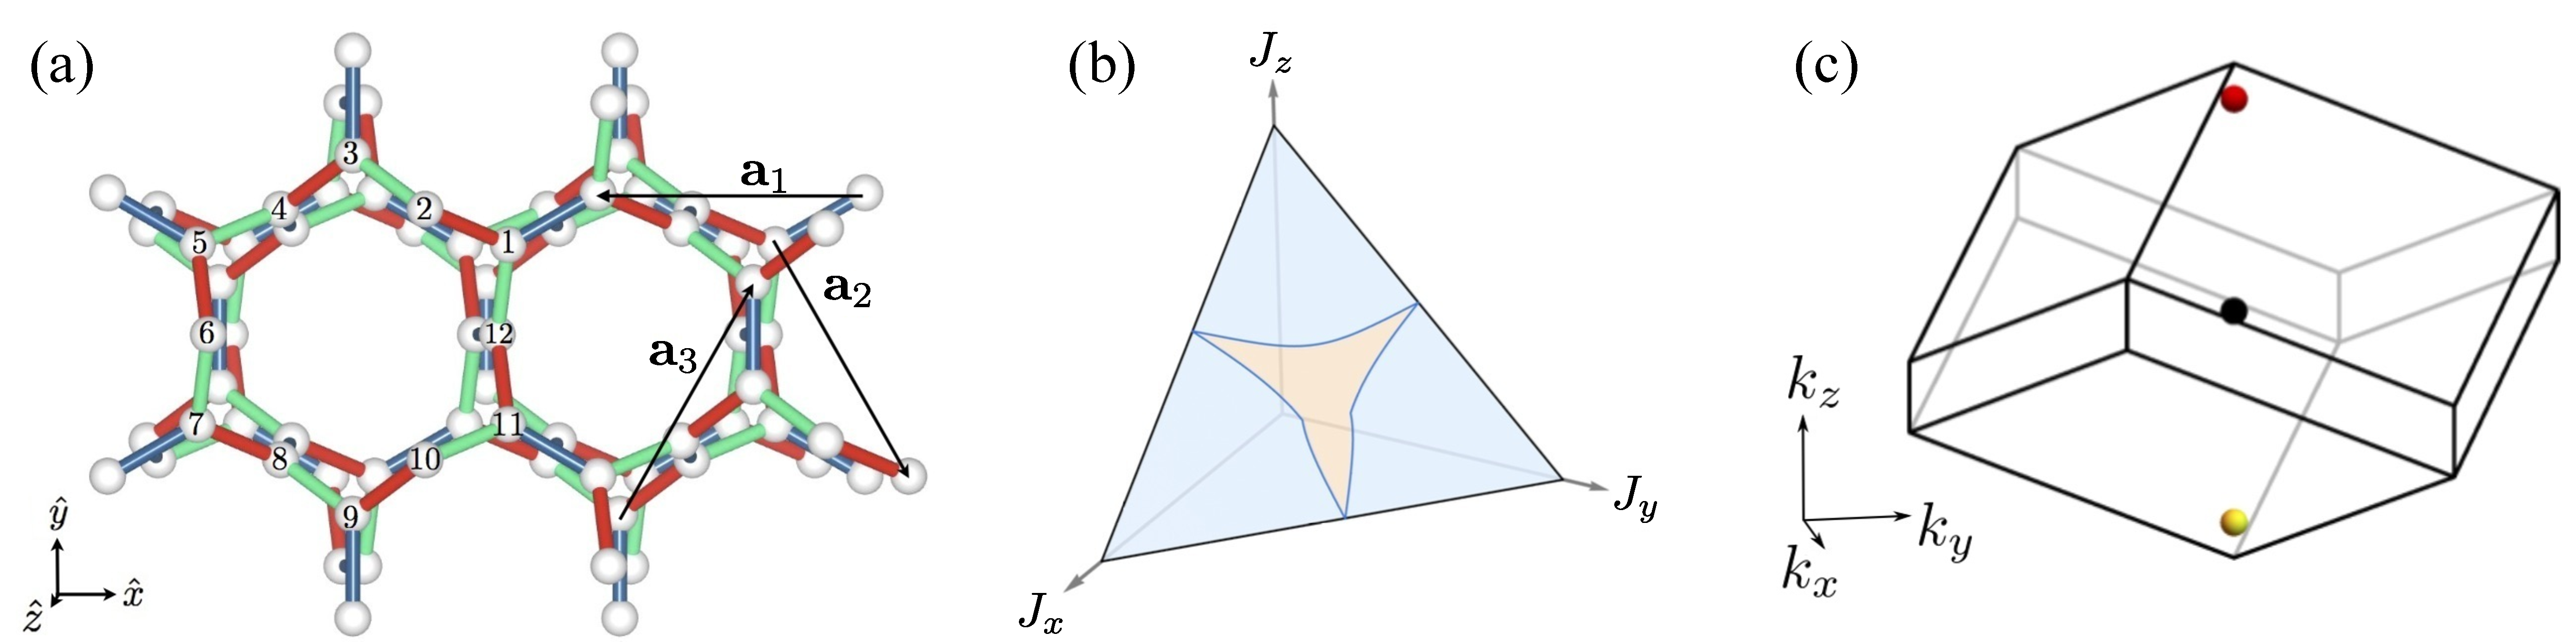
\includegraphics[width=\linewidth]{./chapter06/9_3aPanel.pdf}
	\caption{
		(a) Unit cell and translation vectors for the Kitaev model on the deformed version of lattice (9,3)a.
		(b) Ground state flux phase diagram for lattice (9,3)a.
		(c) Fermionic ground state phase diagram for lattice (9,3)a.
		The orange and blue shaded regions indicate the gapless and gapped spin liquid phases, respectively.
		The data points denoting these two phases were obtained from the corresponding Berry flux calculation.
		The phase boundary is a composite of Berry flux data and gap closing data, as described in the main text.
	}
	\label{fig:chapter06_9_3aPanel}
\end{figure}
%

The lattice is seen to possess a $C_3$ symmetry with rotation axis in the middle of the twelve-site unit cell pointing in the $\hat{e}_z$-direction.
There are three mirror planes which cut through the $z$-type bonds and act to map $x$- and $y$-type bonds onto one another by mapping $\ba_2 \leftrightarrow \ba_3$, $\ba_3 \leftrightarrow \ba_1$ or $\ba_1 \leftrightarrow \ba_2$.
Finally, the lattice is inversion symmetric with multiple, unique inversion centers.
All inversion symmetries map bonds of a given type to the same type of bond.
The first inversion center lies at the center of the twelve-site unit cell, whereas the others are located at the midpoint of the line connecting the aforementioned inversion centers from neighboring unit cells.


%
%
%%%%%%%%%%%%%%%%%%%%%%%%%%%%%%%%%%%%%%%%%%%%%%%%%%%%%%%%%%%%%%%%%%%%%%%%%%%%%%%%%%%%%%%%
\section{Ground state flux configurations}
\label{section:chapter06_Fluxes}
%%%%%%%%%%%%%%%%%%%%%%%%%%%%%%%%%%%%%%%%%%%%%%%%%%%%%%%%%%%%%%%%%%%%%%%%%%%%%%%%%%%%%%%%
%
%
%%%%%%%%%%%%%%%%%%%%%%%%%%%%%%%%%%%%%%%%%%%%%%%%%%%%%%%%%%%%%%%%%%%%%%%%%%%%%%%%%%%%%%%%
\subsection{Quantum Monte Carlo simulations}
\label{section:chapter06_QMC}
%%%%%%%%%%%%%%%%%%%%%%%%%%%%%%%%%%%%%%%%%%%%%%%%%%%%%%%%%%%%%%%%%%%%%%%%%%%%%%%%%%%%%%%%
%
%
As the quantum Monte Carlo (QMC) simulations of the Kitaev model for lattice (9,3)a were not performed by the author of this work, but rather by his collaborators P.~A. Mishchenko and Y. Kato, a detailed explanation of the methods used will not be provided here.
However, in order to frame the remainder of this work, this section will explain the basic ideas behind the simulations.

Due to the bond-dependent interactions of the Kitaev Hamiltonian
%
\begin{equation}
	\op{H}_{\rm Kitaev} = -J_x \sum_{x {\rm -links}} \sigma_j^x \sigma_k^x - J_y \sum_{y {\rm -links}} \sigma_j^y \sigma_k^y - J_z \sum_{z {\rm -links}} \sigma_j^z \sigma_k^z,
\end{equation}
%
the usual spin QMC methods based on the Suzuki-Trotter decomposition suffer from the negative sign problem and cannot be used~\cite{NasuPRL2014}.
However, in Chapter~\ref{chapter:KitaevHoneycombModel} it was seen that the Kitaev Hamiltonian may be reframed as a free Majorana Hamiltonian in the background of a static \ZZ~gauge field.
The fermionic Kitaev Hamiltonian in a fixed gauge sector may be straightforwardly diagonalized and the resulting eigenbasis used in the QMC simulations in order to avoid the sign problem~\cite{NasuPRL2014}.
In practice, rather than using the Majorana representations seen in Chapters~\ref{chapter:KitaevHoneycombModel} and~\ref{chapter:ProjectiveSymmetryGroup}, the model is solved via Jordan-Wigner transformation~\cite{ChenPRB2007,FengPRL2007,ChenJPA2008}, resulting in the free Majorana Hamiltonian
%
\begin{equation}
	\op{H}(\{\eta\}) = i J_x \sum_{x {\rm -links}} \eta_{jk} c_j c_k + i J_y \sum_{y {\rm -links}} c_j c_k + i J_z \sum_{z {\rm -links}} c_j c_k,
	\label{eq:chapter06_JWHamiltonian}
\end{equation}
%
where a convention for the orientation of bonds must be fixed and $\eta_{jk} = \pm 1$ is a \ZZ~degree of freedom living only on the $x$-type bonds.

The QMC simulation may now be performed by sampling the classical, Ising-like variables $\eta_{ij}$, where the Monte Carlo weight for a given configuration of $\{\eta\}$ is obtained by the exact diagonalization of the Majorana fermions in Hamiltonian~\eqref{eq:chapter06_JWHamiltonian}.
In practice, other numerical "tricks" are employed to access larger system sizes and lower temperatures.
For example, the simulations do not use exact diagonalization to determine the Monte Carlo weight of a given configuration of $\{\eta\}$, rather, they employ a kernel polynomial method~\cite{WeisseRMP2006,WeissePRL2009} to approximate the difference in free energy between two configurations, reducing the numerical cost from $\mathcal{O}(N^4)$ to $\mathcal{O}(N^2)$, where $N$ is the total number of spins~\cite{MischenkoPRB2017}.
Additionally, the simulations utilized feedback-optimized parallel tempering methods in order to access lower temperatures~\cite{TrebstPRE2004,KatzgraberJSM2006}.


%
%
%%%%%%%%%%%%%%%%%%%%%%%%%%%%%%%%%%%%%%%%%%%%%%%%%%%%%%%%%%%%%%%%%%%%%%%%%%%%%%%%%%%%%%%%
\subsection{Results}
\label{section:chapter06_QMCResults}
%%%%%%%%%%%%%%%%%%%%%%%%%%%%%%%%%%%%%%%%%%%%%%%%%%%%%%%%%%%%%%%%%%%%%%%%%%%%%%%%%%%%%%%%
%
%
%
\begin{figure}[tb]
	\centering
	\includegraphics[width=\linewidth]{./chapter06/9_3aFluxConfigurations.pdf}
	\caption{
		Flux configurations for lattice (9,3)a where the flux loops are represented by colored spheres.
		Loops of length 9 are colored white or black corresponding to $+\pi/2$-flux or $-\pi/2$-flux, respectively.
		Loops of length 12 are colored blue or red corresponding to $\pi$-flux or $0$-flux, respectively.
		(a) Single flux unit cell of lattice (9,3)a.
		(b) Flux configuration A0F.
		(c) Flux configuration SII.
		(d) Flux configuration SI.
		(e) Flux configuration AF.
		(f) Flux configuration AFII.
	}
	\label{fig:chapter06_9_3aFluxConfigurations}
\end{figure}
%
In addition to the QMC simulations described above, a number of potential ground state flux configurations were found from effective models obtained in the various limits of anisotropic exchange couplings via perturbation theory.
A combination of the QMC results along with a straightforward variational approach using the aforementioned trial flux configurations was used to determine the ground state flux configuration as a function of exchange couplings.
The resulting ground state flux phase diagram is pictured in Figure~\ref{fig:chapter06_9_3aPanel}~(b).
As can be seen from the figure, the ground state of the Kitaev model on lattice (9,3)a exhibits a variety of different flux phases.
It turns out that the SII and A0F flux phases (depicted in Figures~\ref{fig:chapter06_9_3aFluxConfigurations}~(b) and (c), respectively) correspond to fully gapped quantum spin liquid ground states, whereas the SI, AF and AFII flux phases (depicted in Figures~\ref{fig:chapter06_9_3aFluxConfigurations}~(d), (e) and (f), respectively) host both gapped and gapless quantum spin liquid ground states depending on the exact choice of coupling strengths.
The distinction lies in the gapped/gapless nature of the fermionic quasiparticle excitations which are explored in detail in the remainder of this chapter.


%
%
%%%%%%%%%%%%%%%%%%%%%%%%%%%%%%%%%%%%%%%%%%%%%%%%%%%%%%%%%%%%%%%%%%%%%%%%%%%%%%%%%%%%%%%%
\section{Gapless spin liquids}
\label{section:chapter06_GaplessSpinLiquids}
%%%%%%%%%%%%%%%%%%%%%%%%%%%%%%%%%%%%%%%%%%%%%%%%%%%%%%%%%%%%%%%%%%%%%%%%%%%%%%%%%%%%%%%%
%
%
%%%%%%%%%%%%%%%%%%%%%%%%%%%%%%%%%%%%%%%%%%%%%%%%%%%%%%%%%%%%%%%%%%%%%%%%%%%%%%%%%%%%%%%%
\subsection{Fermionic phase diagram}
\label{section:chapter06_GaplessPhaseDiagram}
%%%%%%%%%%%%%%%%%%%%%%%%%%%%%%%%%%%%%%%%%%%%%%%%%%%%%%%%%%%%%%%%%%%%%%%%%%%%%%%%%%%%%%%%
%
%
Given the ground state \textit{flux} phase diagram discussed in Section~\ref{section:chapter06_Fluxes}, the \textit{fermionic} ground state phase diagram may be mapped out by assigning the correct flux configuration for a given choice of exchange couplings and checking the resulting fermionic spectrum.
In order to efficiently determine whether the fermionic quasiparticles are gapped or gapless at a given point in the phase diagram, the non-Abelian Berry curvature is integrated over two-dimensional planes which cut through the three-dimensional Brillouin zone, \ie, by fixing one component of the momentum and integrating over the other two~\cite{FukuiJPS2005}.
This is analogous to what was described in Section~\ref{section:chapter05_8_3b} to calculate the chirality of Weyl nodes.

For those planes on which the fermionic spectrum is gapped, the result is a quantized Chern number.
In a Weyl spin liquid phase, the Chern number jumps discontinuously as the plane passes through a Weyl node by an amount equal to the charge of that Weyl node.
In general, the Berry curvature is ill-defined for a plane on which the fermionic spectrum is gapless.
In the case that there is a one- or two-dimensional nodal manifold, the result is a range of momentum values for which the Berry flux is ill-defined and fluctuates wildly.

With this information, it may be determined whether a given point in the phase diagram corresponds to a gapped or gapless fermionic spectrum.
If the Berry flux is everywhere vanishing, the fermions must be gapped throughout the entire Brillouin zone.
However, if at any point the Berry flux is \textit{non-zero} -- whether it takes a non-vanishing quantized Chern number or fluctuates wildly -- the fermionic spectral gap must close somewhere.
For those regions of the phase diagram where the gap closing occurs at a high-symmetry point, the resolution of the phase diagram data was greatly increased by checking whether or not the gap closes at that point for a given choice of couplings. 
The resulting fermionic ground state phase diagram is pictured in  Figure~\ref{fig:chapter06_9_3aPanel}~(c).

In Figure~\ref{fig:chapter06_9_3aPanel}, the ground state phase diagrams for the \ZZ~gauge field and the fermions are pictured separately for clarity.
Composites of the two phase diagrams appear below, however, in the context of the different gapless spin liquid phases.
Whereas the flux phases A0F and SII are seen to be fully gapped, the flux phases SI, AF and AFII have both gapped and gapless regions.
In the following sections, the nature of the gapless regions are discussed for the flux phases SI, AF and AFII.
In all cases, the elementary unit cell is doubled in all directions to accommodate the gauge \textit{Ansatz}.


%
%
%%%%%%%%%%%%%%%%%%%%%%%%%%%%%%%%%%%%%%%%%%%%%%%%%%%%%%%%%%%%%%%%%%%%%%%%%%%%%%%%%%%%%%%%
\subsection{SI flux phase}
\label{section:chapter06_SIPhase}
%%%%%%%%%%%%%%%%%%%%%%%%%%%%%%%%%%%%%%%%%%%%%%%%%%%%%%%%%%%%%%%%%%%%%%%%%%%%%%%%%%%%%%%%
%
%
\subsubsection{Gauge structure and projective symmetries}
%
%
In the SI flux configuration, all loops of length 12 are assigned $\pi$-flux, whereas the loops of length 9 are assigned $\pm \pi/2$-flux according to their position in the unit cell.
A representation of the SI flux configuration is pictured in Figure~\ref{fig:chapter06_9_3aFluxConfigurations}~(d).
Although the flux configuration has the same translation symmetry as the lattice, the unit cell is doubled in all directions to accommodate the gauge \textit{Ansatz}.

The arrangement of fluxes is seen to respect inversion symmetry for \textit{all} inversion centers, however, it breaks $C_3$ symmetry and two out of three mirror symmetries.
By virtue of lattice (9,3)a being non-bipartite, the flux configuration necessarily breaks time-reversal symmetry (see Section~\ref{section:chapter05_9_3a} for details).

The projective symmetry operators have not been explicitly constructed due to the enormous 96 site unit cell, however, the fermionic spectrum is seen \textit{not} to possess any finite nesting vectors.
The relevant energy relations are, thus, given by
%
\begin{equation}
	E_{\alpha}(\bk) = -E_{\beta}(-\bk) \qquad {\rm and} \qquad E_{\alpha}(\bk) = E_{\gamma}(-\bk),
\end{equation}
%
due to particle-hole and inversion symmetry, respectively.
Due to the lack of a projective time-reversal operator, the momentum space Hamiltonian matrix has the general form
%
\begin{equation}
	H(\bk) = 
		\begin{pmatrix}
			0			&		 & A(\bk) \\
						& \ddots & 		  \\
			A\dag(\bk)	&		 & 0
		\end{pmatrix},
\end{equation}
%
\ie, it is an inversion symmetric band Hamiltonian.


%
%
\subsubsection{Majorana band structure}
%
%
%
\begin{figure}[tb]
	\centering
	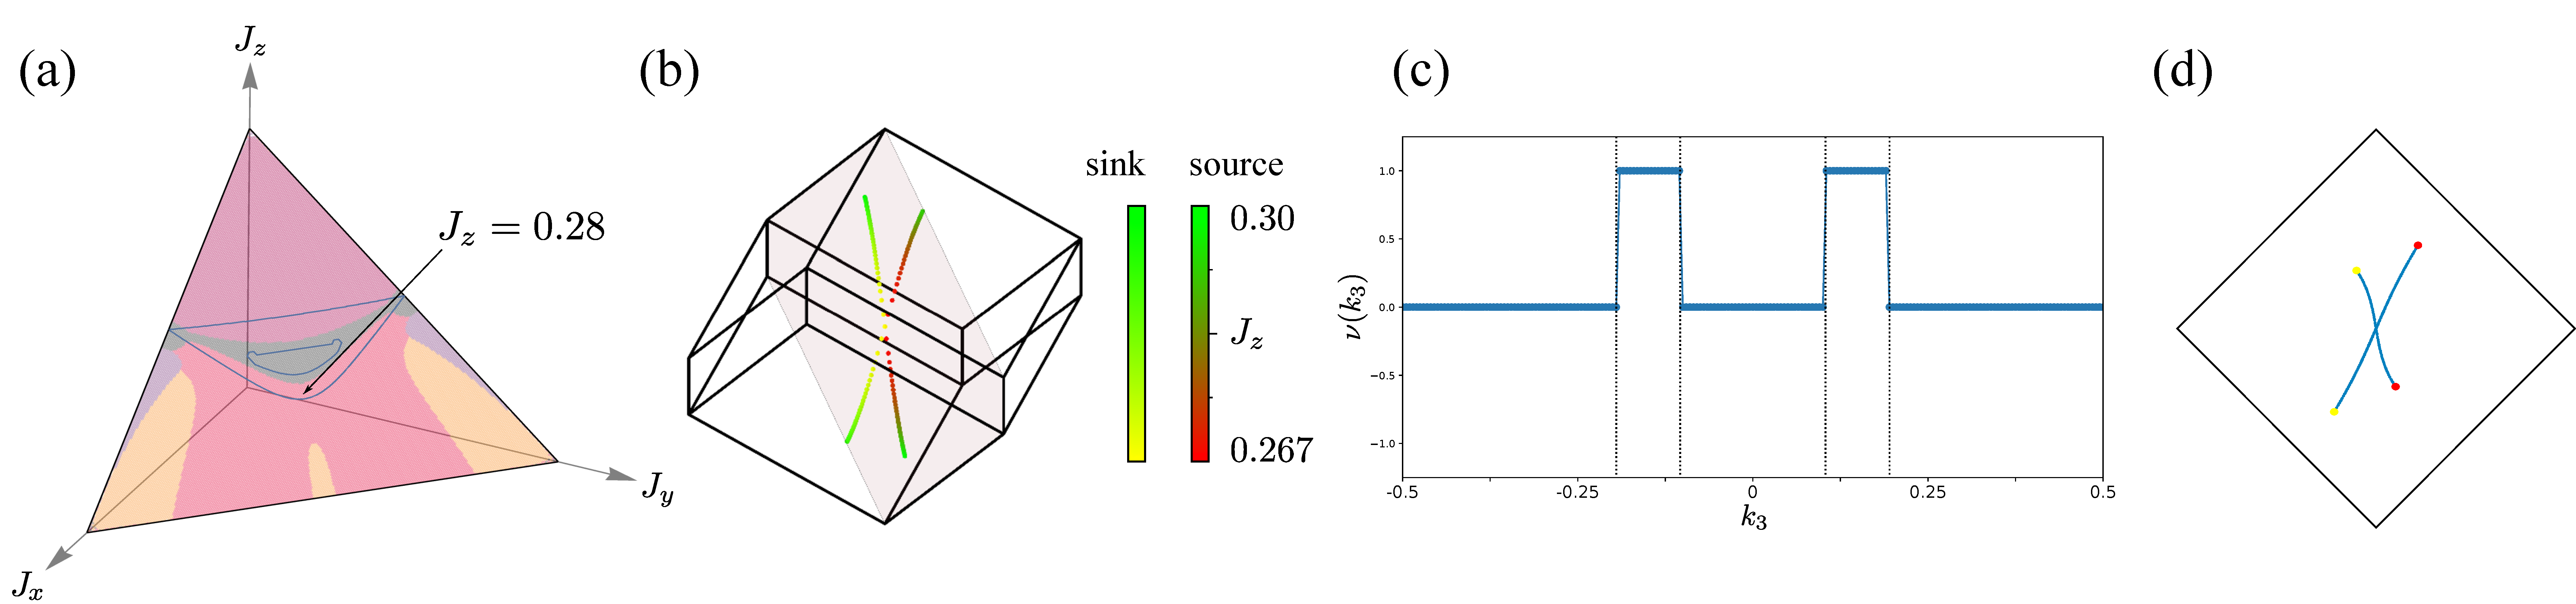
\includegraphics[width=\linewidth]{./chapter06/9_3a_SIPanel.pdf}
	\caption{
		(a) Gapless SI phase for lattice (9,3)a.
		The arrow indicates the point $(J_x, J_y, J_z) = (0.36, 0.36, 0.28)$.
		For fixed $J_x = J_y = (1 - J_z)/2$, the gapless portion of the SI phase begins for $J_z \gtrsim 0.267$ where the gap closes and ends for $J_z \gtrsim 0.3$ where the ground state flux configuration switches from SI to AFII.
		(b) Evolution of Weyl nodes for lattice (9,3)a for varied coupling constants $0.267 \leq J_z \leq 0.30$ with $J_x = J_y = (1 - J_z)/2$.
		The shaded region indicates the remaining mirror plane for the SI flux phase with $J_x = J_y$.
		(c) Chern number as a function of momentum $k_3$ for the choice of couplings $(J_x, J_y, J_z) = (0.36, 0.36, 0.28)$.
		The dashed lines indicate the $k_3$-component of the Weyl node positions.
		(d) Corresponding Fermi arcs in the 001-surface Brillouin zone for $(J_x, J_y, J_z) = (0.36, 0.36, 0.28)$.
	}
	\label{fig:chapter06_SIPanel}
\end{figure}
%
As discussed in Chapter~\ref{chapter:ClassificationOfKSL}, the presence of trivially implemented inversion symmetries, \ie, with vanishing nesting vector, prohibits the formation of stable Fermi surfaces.
Furthermore, the absence of time-reversal symmetry prevents the formation of nodal lines protected by the one-dimensional winding number discussed in Section~\ref{section:chapter05_8_3c}.
However, the combination of particle-hole and inversion symmetries allows for the presence of topologically protected Weyl nodes pinned to zero energy.

Indeed, diagonalizing the concrete Hamiltonian for lattice (9,3)a in the SI flux configuration reveals an extended gapless Weyl spin liquid phase (see Figure~\ref{fig:chapter06_SIPanel}~(a)).
Restricting the exchange couplings to the line $J_x = J_y = (1 - J_z)/2$, the gapless portion of the SI phase runs from $J_z \approx 0.267$, where the gap closes, to $J_z \approx 0.3$, where the ground state flux configuration switches from SI to AFII.
For $J_z \approx 0.267$, two positively charged and two negatively charged Weyl nodes simultaneously appear at the $\Gamma$-point.
As $J_z$ is increased further, the Weyl nodes split apart.
For $J_x = J_y$, the Weyl nodes are pinned to the single mirror plane which is \textit{not} broken by the SI flux configuration.

Figure~\ref{fig:chapter06_SIPanel}~(b) shows the evolution of the Weyl nodes in the 3D Brillouin zone as the exchange couplings are varied for $0.276 \leq J_z \leq 0.30$ with $J_x = J_y = (1 - J_z)/2$, along with the aforementioned mirror plane.
The trajectory of negatively charged Weyl nodes changes color from yellow to green as $J_z$ is increased, whereas the trajectory of positively charged Weyl nodes changes from red to green.
In Figure~\ref{fig:chapter06_SIPanel}~(c) is plotted the Chern number as a function of $k_3 = \bk \cdot \bq_3 / 2\pi$ for $(J_x, J_y, J_z) = (0.36, 0.36, 0.28)$, indicating the charge of the Weyl nodes in the bulk.
The corresponding Fermi arcs in the 001-surface Brillouin zone for the same choice of couplings are plotted in Figure~\ref{fig:chapter06_SIPanel}~(d).


%
%
%%%%%%%%%%%%%%%%%%%%%%%%%%%%%%%%%%%%%%%%%%%%%%%%%%%%%%%%%%%%%%%%%%%%%%%%%%%%%%%%%%%%%%%%
\subsection{AF flux phase}
\label{section:chapter06_AFPhase}
%%%%%%%%%%%%%%%%%%%%%%%%%%%%%%%%%%%%%%%%%%%%%%%%%%%%%%%%%%%%%%%%%%%%%%%%%%%%%%%%%%%%%%%%
%
%
\subsubsection{Gauge structure and projective symmetries}
%
%
In the AF flux configuration, all loops of length 12 are assigned $\pi$-flux, whereas the loops of length 9 are assigned $\pm \pi/2$-flux according to their position in the unit cell.
A representation of the AF flux configuration is pictured in Figure~\ref{fig:chapter06_9_3aFluxConfigurations}~(e).
Although the flux configuration has the same translation symmetry as the lattice, the unit cell is doubled in all directions to accommodate the gauge \textit{Ansatz}.

The arrangement of fluxes is seen to respect inversion symmetry for \textit{all} inversion centers, as well as the $C_3$-rotation symmetry and all mirror symmetries.
By virtue of lattice (9,3)a being non-bipartite, the flux configuration necessarily breaks time-reversal symmetry (see Section~\ref{section:chapter05_9_3a} for details).

The projective symmetry operators have not been explicitly constructed due to the enormous 96 site unit cell, however, the fermionic spectrum is seen \textit{not} to possess any finite nesting vectors.
The relevant energy relations are, thus, given by
%
\begin{equation}
	E_{\alpha}(\bk) = -E_{\beta}(-\bk) \qquad {\rm and} \qquad E_{\alpha}(\bk) = E_{\gamma}(-\bk),
\end{equation}
%
due to particle-hole and inversion symmetry, respectively.
Due to the lack of a projective time-reversal operator, the momentum space Hamiltonian matrix has the general form
%
\begin{equation}
	H(\bk) = 
		\begin{pmatrix}
			0			&		 & A(\bk) \\
			& \ddots & 		  \\
			A\dag(\bk)	&		 & 0
		\end{pmatrix},
\end{equation}
%
\ie, it is an inversion symmetric band Hamiltonian.


%
%
\subsubsection{Majorana band structure}
%
%
%
\begin{figure}[tb]
	\centering
	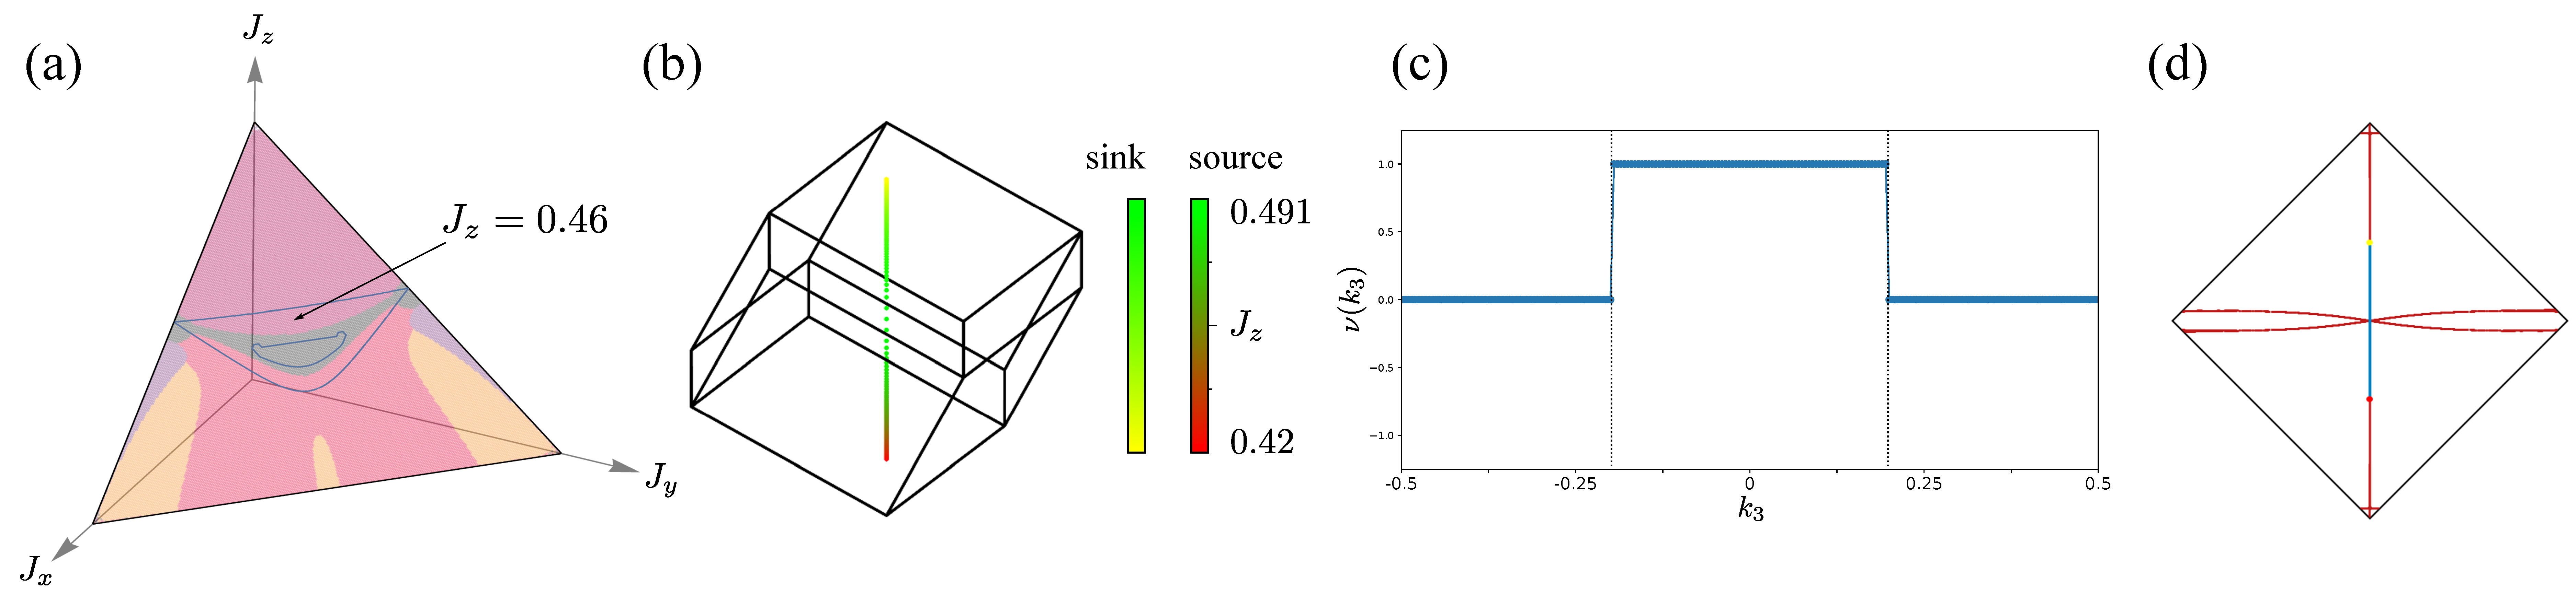
\includegraphics[width=\linewidth]{./chapter06/9_3a_AFPanel.pdf}
	\caption{
		(a) Gapless AF phase for lattice (9,3)a.
		The arrow indicates the point $(J_x, J_y, J_z) = (0.27, 0.27, 0.46)$.
		For fixed $J_x = J_y = (1 - J_z)/2$, the gapless portion of the AF phase begins for $J_z \gtrsim 0.42$, where the ground state flux configuration switches from AFII to AF, and ends for $J_z \gtrsim 0.491$, where the gap reopens.
		(b) Evolution of Weyl nodes for lattice (9,3)a for varied coupling constants $0.42 \leq J_z \leq 0.491$ with $J_x = J_y = (1 - J_z)/2$.
		(c) Chern number as a function of momentum $k_3$ for the choice of couplings $(J_x, J_y, J_z) = (0.27, 0.27, 0.46)$.
		The dashed lines indicate the $k_3$-component of the Weyl node positions.
		(d) Corresponding Fermi arc in the 001-surface Brillouin zone for $(J_x, J_y, J_z) = (0.27, 0.27, 0.46)$ denoted in blue.
		Additional surface states are marked in red and are discussed in the main text.
	}
	\label{fig:chapter06_AFPanel}
\end{figure}
%
As is the case for the SI phase discussed above, the presence of trivially implemented inversion symmetries, \ie, with vanishing nesting vector, prohibits the formation of stable Fermi surfaces.
Furthermore, the absence of time-reversal symmetry prevents the formation of nodal lines protected by the one-dimensional winding number discussed in Section~\ref{section:chapter05_8_3c}.
However, the combination of particle-hole and inversion symmetries allows for the presence of topologically protected Weyl nodes pinned to zero energy.

Indeed, diagonalizing the concrete Hamiltonian for lattice (9,3)a in the AF flux configuration reveals an extended gapless Weyl spin liquid phase (see Figure~\ref{fig:chapter06_AFPanel}~(a)).
Restricting the exchange couplings to the line $J_x = J_y = (1 - J_z)/2$, the gapless portion of the AF phase runs from $J_z \approx 0.42$, where the ground state flux configuration switches from AFII to AF, to $J_z \approx 0.491$, where the Weyl nodes gap out.
For $0.42 < J_z \lesssim 0.491$, two oppositely charged Weyl nodes are pinned to the $C_3$-invariant axis while $J_x = J_y$.
As $J_z$ is increased, the two Weyl nodes move towards each other until they eventually meet at the $\Gamma$-point for $J_z \approx 0.491$ and mutually annihilate.

Figure~\ref{fig:chapter06_AFPanel}~(b) shows the evolution of the Weyl nodes in the 3D Brillouin zone as the exchange couplings are varied for $0.42 \leq J_z \leq 0.491$ with $J_x = J_y = (1 - J_z)/2$.
The trajectory of negatively charged Weyl nodes changes color from yellow to green as $J_z$ is increased, whereas the trajectory of positively charged Weyl nodes changes from red to green.
In Figure~\ref{fig:chapter06_AFPanel}~(c) is plotted the Chern number as a function of $k_3 = \bk \cdot \bq_3 / 2\pi$ for $(J_x, J_y, J_z) = (0.27, 0.27, 0.46)$, indicating the charge of the Weyl nodes in the bulk.
The corresponding Fermi arc in the 001-surface Brillouin zone for the same choice of couplings are plotted in Figure~\ref{fig:chapter06_AFPanel}~(d).

In addition to the Fermi arc which terminates at the projection of the Weyl nodes in the surface Brillouin zone, there appear additional line-like surface states which form incontractible loops.
These can be seen as remnants of Fermi arcs due to Weyl nodes which are gapped out in this part of the phase diagram.
If the AF flux configuration is extended beyond its range of validity, \ie, for $J_z \lesssim 0.42$ with $J_x = J_y$, one finds the existence of an additional six Weyl nodes.
These Weyl nodes emerge from the $\Gamma$-point at $J_z \approx 0.294$ and move away from one another as $J_z$ is increased, always pinned to the three mirror planes.
At $J_z \approx 0.414$, the six Weyl nodes once again meet and annihilate at the $\Gamma$-point.
However, as they do so, they trace out incontractible loops across the Brillouin zone.
In Figure~\ref{fig:chapter06_AFPanel2}~(a) and (b) are pictured the evolution of these six additional Weyl nodes (excluding the two Weyl nodes on the $C_3$-invariant axis mentioned in the previous paragraph) in the bulk Brillouin zone and projected down to the 001-surface Brillouin zone, respectively.
Here can be seen the incontractible loops along which they travel before gapping out.
%
\begin{figure}[tb]
	\centering
	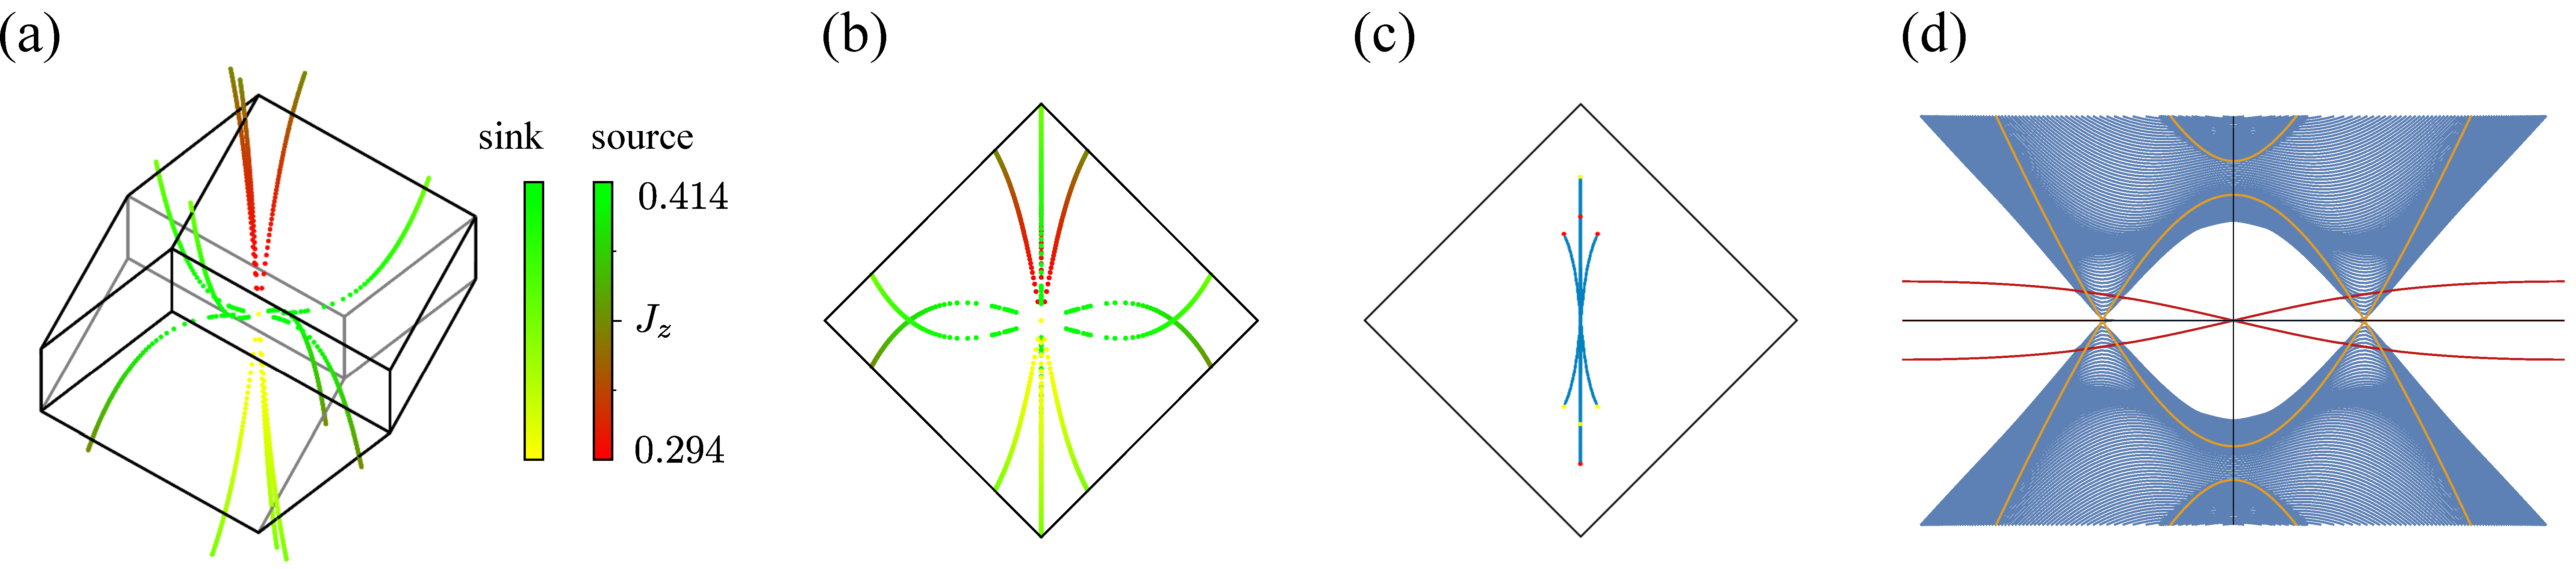
\includegraphics[width=\linewidth]{./chapter06/9_3a_AFPanel2.pdf}
	\caption{
		(a) Evolution of Weyl nodes for lattice (9,3)a for varied coupling constants $0.294 \leq J_z \leq 0.414$ with $J_x = J_y = (1 - J_z)/2$.
		The two Weyl nodes on the $C_3$-invariant axis are not shown for clarity.
		(b) Evolution of Weyl nodes for lattice (9,3)a for varied coupling constants $0.294 \leq J_z \leq 0.414$ with $J_x = J_y = (1 - J_z)/2$ projected down to the 001-surface Brillouin zone.
		The two Weyl nodes on the $C_3$-invariant axis are not shown for clarity.
		(c) Corresponding Fermi arcs in the 001-surface Brillouin zone for $(J_x, J_y, J_z) = (0.345, 0.345, 0.31)$.
		This includes the Weyl nodes which lie on the $C_3$-invariant axis along with their corresponding Fermi arc.
		(d) Band structures for $J_z = 0.46$.
		The bulk band structure along the $C_3$-invariant axis is plotted in yellow showing the two Weyl nodes.
		The band structure for the slab geometry along the projection of the $C_3$ axis to the surface Brillouin zone is plotted in blue and red.
		Here in blue are seen the projection of the two Weyl nodes as well as the Fermi arc which connects them.
		In red are plotted the bands responsible for the remaining surface states left over from the other Weyl nodes which are gapped out for $J_z \approx 0.414$.
	}
	\label{fig:chapter06_AFPanel2}
\end{figure}
%

A consequence of their trajectories through the Brillouin zone is that their corresponding Fermi arcs (pictured in Figure~\ref{fig:chapter06_AFPanel2}~(c)), rather than shrinking to a point and gapping out with the Weyl nodes, are stretched out along similar incontractible loops.
The result is that, while the Weyl nodes responsible for the surface states gap out, the surface states themselves remain behind (as can be seen in Figure~\ref{fig:chapter06_AFPanel}~(d) pictured in red).
Pictured in Figure~\ref{fig:chapter06_AFPanel2}~(d) is a composite of the bulk and slab geometry band structures for $J_z = 0.46$ computed along the $C_3$-invariant axis and its projection to the 001-surface Brillouin zone, respectively.
Here can be seen the Fermi arcs in blue which terminate at the projection of the Weyl nodes to the surface Brillouin zone at which point they dive back into the bulk.
In red, however, are pictured the remnant surface bands from the Weyl nodes which have been gapped out.
These bands are seen to be entirely disconnected from the bulk band structure.


%
%
%%%%%%%%%%%%%%%%%%%%%%%%%%%%%%%%%%%%%%%%%%%%%%%%%%%%%%%%%%%%%%%%%%%%%%%%%%%%%%%%%%%%%%%%
\subsection{AFII flux phase}
\label{section:chapter06_AFIIPhase}
%%%%%%%%%%%%%%%%%%%%%%%%%%%%%%%%%%%%%%%%%%%%%%%%%%%%%%%%%%%%%%%%%%%%%%%%%%%%%%%%%%%%%%%%
%
%
\subsubsection{Gauge structure and projective symmetries}
%
%
In the AFII flux configuration, all loops of length 12 are assigned $\pi$-flux, whereas the loops of length 9 are assigned $\pm \pi/2$-flux according to their position in the unit cell.
A representation of the AFII flux configuration is pictured in Figure~\ref{fig:chapter06_9_3aFluxConfigurations}~(f).
The AFII flux configuration requires a doubling of the unit cell in all directions.

The arrangement of fluxes is seen to respect $C_3$-rotation symmetry, all mirror symmetries and inversion symmetry through the point at the center of the unit cell, however, it breaks all other inversion symmetries.
By virtue of lattice (9,3)a being non-bipartite, the flux configuration necessarily breaks time-reversal symmetry (see Section~\ref{section:chapter05_9_3a} for details).
Note, however, that the combination of broken time-reversal with the broken inversion symmetry is indeed a symmetry of the AFII flux configuration.

The projective symmetry operators have not been explicitly constructed due to the enormous 96 site unit cell, however, the fermionic spectrum is seen \textit{not} to possess any finite nesting vectors.
The relevant energy relations are, thus, given by
%
\begin{equation}
	E_{\alpha}(\bk) = -E_{\beta}(-\bk) \qquad {\rm and} \qquad E_{\alpha}(\bk) = E_{\gamma}(-\bk),
\end{equation}
%
due to particle-hole and inversion symmetry, respectively.
Due to the lack of a projective time-reversal operator, the momentum space Hamiltonian matrix has the general form
%
\begin{equation}
	H(\bk) = 
		\begin{pmatrix}
			0			&		 & A(\bk) \\
			& \ddots & 		  \\
			A\dag(\bk)	&		 & 0
		\end{pmatrix},
\end{equation}
%
\ie, it is an inversion symmetric band Hamiltonian.
\newpage


%
%
\subsubsection{Majorana band structure}
%
%
%
\begin{figure}[tb]
	\centering
	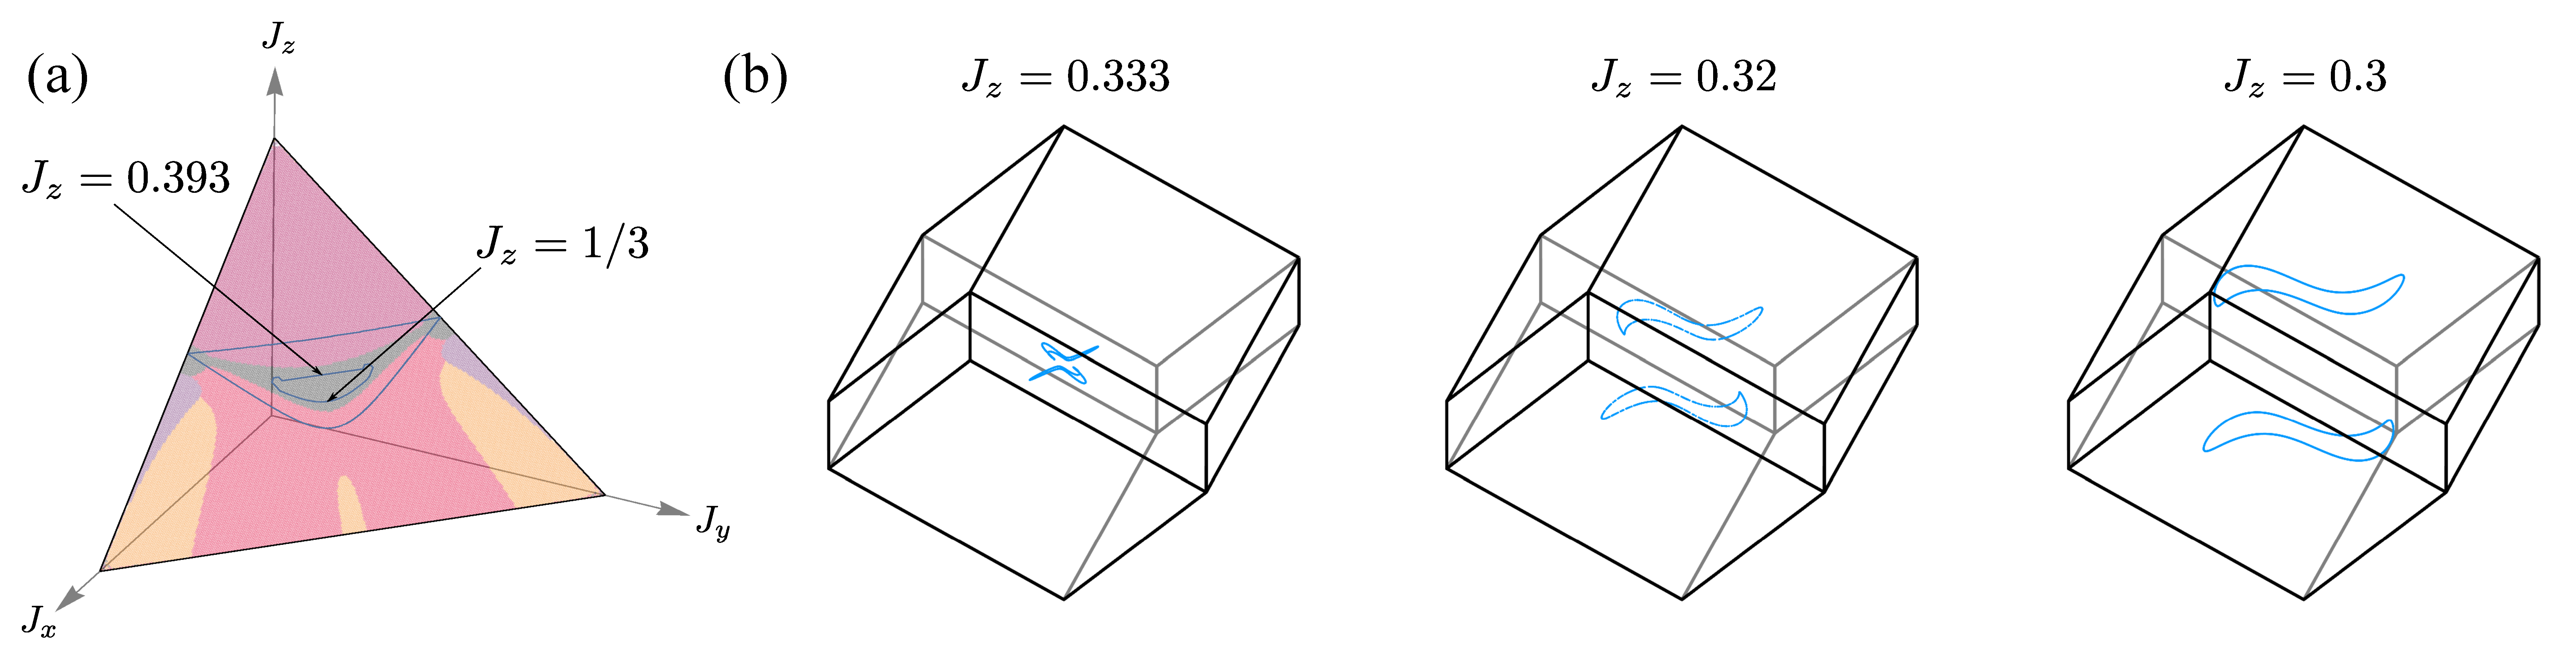
\includegraphics[width=\linewidth]{./chapter06/9_3a_AFIIPanel1.pdf}
	\caption{
		(a) Gapless AF phase for lattice (9,3)a.
		The arrows indicates the points $(J_x, J_y, J_z) = (1/3, 1/3, 1/3)$ and $(J_x, J_y, J_z) \approx (0.304, 0.304, 0.393)$.
		For fixed $J_x = J_y = (1 - J_z)/2$, the gapless portion of the AFII phase runs from $J_z \approx 0.3$, where the ground state flux configuration switches from SI to AFII, to $J_z \approx 0.42$, where the  ground state flux configuration switches from AFII to AF, with a region in between $1/3 < J_z \lesssim 0.392$ for which the spectrum is fully gapped.
		(b) Evolution of nodal lines for several values of $J_z < 1/3$.
	}
	\label{fig:chapter06_AFIIPanel}
\end{figure}
%
As already discussed above, the presence of trivially implemented inversion symmetry, \ie, with vanishing nesting vector, prohibits the formation of stable Fermi surfaces.
Furthermore, the absence of time-reversal symmetry prevents the formation of nodal lines protected by the one-dimensional winding number discussed in Section~\ref{section:chapter05_8_3c}.
%
%
%
However, it has been shown that in a system where the combination of inversion and time-reversal is a symmetry, one may define both one- and two-dimensional \ZZ~winding numbers~\cite{KimPRL2015,FangPRB2015}.
The one-dimensional winding number corresponds to a Berry phase of either 0 or $\pi$ acquired upon traversal of a one-dimensional loop and may stabilize nodal lines similarly to what was seen above for the time-reversal invariant spin liquids.
Additionally, pairs of nodal lines can be stabilized by the presence of a \textit{two}-dimensional \ZZ~winding number, \ie, a nodal line may carry a \ZZ~monopole charge defined on a two-dimensional surface which encloses it.
Due to their monopole charge, such nodal lines must always be created and annihilated in pairs rather than being continuously deformed to a point and gapped out in isolation.
Crucially, inversion and time-reversal operations need not individually be symmetries of the system, rather, only the combination of the two.
For lattice (9,3)a, any fixed flux sector breaks time-reversal symmetry spontaneously, however, in the AFII phase where one of the inversion symmetries is broken, the combination of the corresponding inversion operation with time-reversal indeed yields a symmetry of the Hamiltonian.
In this case, such line nodes can be stable.

Diagonalizing the concrete Hamiltonian for lattice (9,3)a in the AFII flux configuration reveals an extended gapless spin liquid phase with gapless excitations corresponding to nodal lines (see Figure~\ref{fig:chapter06_AFIIPanel}~(a)).
Restricting the exchange couplings to the line $J_x = J_y = (1 - J_z)/2$, the gapless portion of the AFII phase runs from $J_z \approx 0.3$, where the ground state flux configuration switches from SI to AFII, to $J_z \approx 0.42$, where the  ground state flux configuration switches from AFII to AF, with a region in between $1/3 < J_z \lesssim 0.392$ for which the spectrum is fully gapped.

At the isotropic point $J_z = 1/3$ there is a fourfold zero energy degeneracy at the $\Gamma$-point which is gapped out as soon as $J_z$ is increased.
However, for $J_z < 1/3$, this fourfold degeneracy is split into two nodal lines which grow larger and move away from each other as $J_z$ is increased further (see Figure~\ref{fig:chapter06_AFIIPanel}~(b)).
Extending the analysis of the AFII flux configuration for $J_z \lesssim 0.3$ where there is a phase transition to the SI flux phase, the nodal lines can be seen to wrap around the Brillouin zone before meeting once more and mutually annihilating at $J_z \approx 0.22$.
Putting the system on a slab geometry, one finds both "drumhead" surface states filling the projection of the nodal lines to the surface Brillouin zone~\cite{ChenNatComm2015,MullenPRL2015} as well as Fermi arc surface states connecting the two projections (see Figure~\ref{fig:chapter06_AFIIPanel3}~(a)) as a result of the \ZZ~monopole charges of the nodal lines~\cite{GorbarPRB2015a,GorbarPRB2015b}.
%
\begin{figure}[tb]
	\centering
	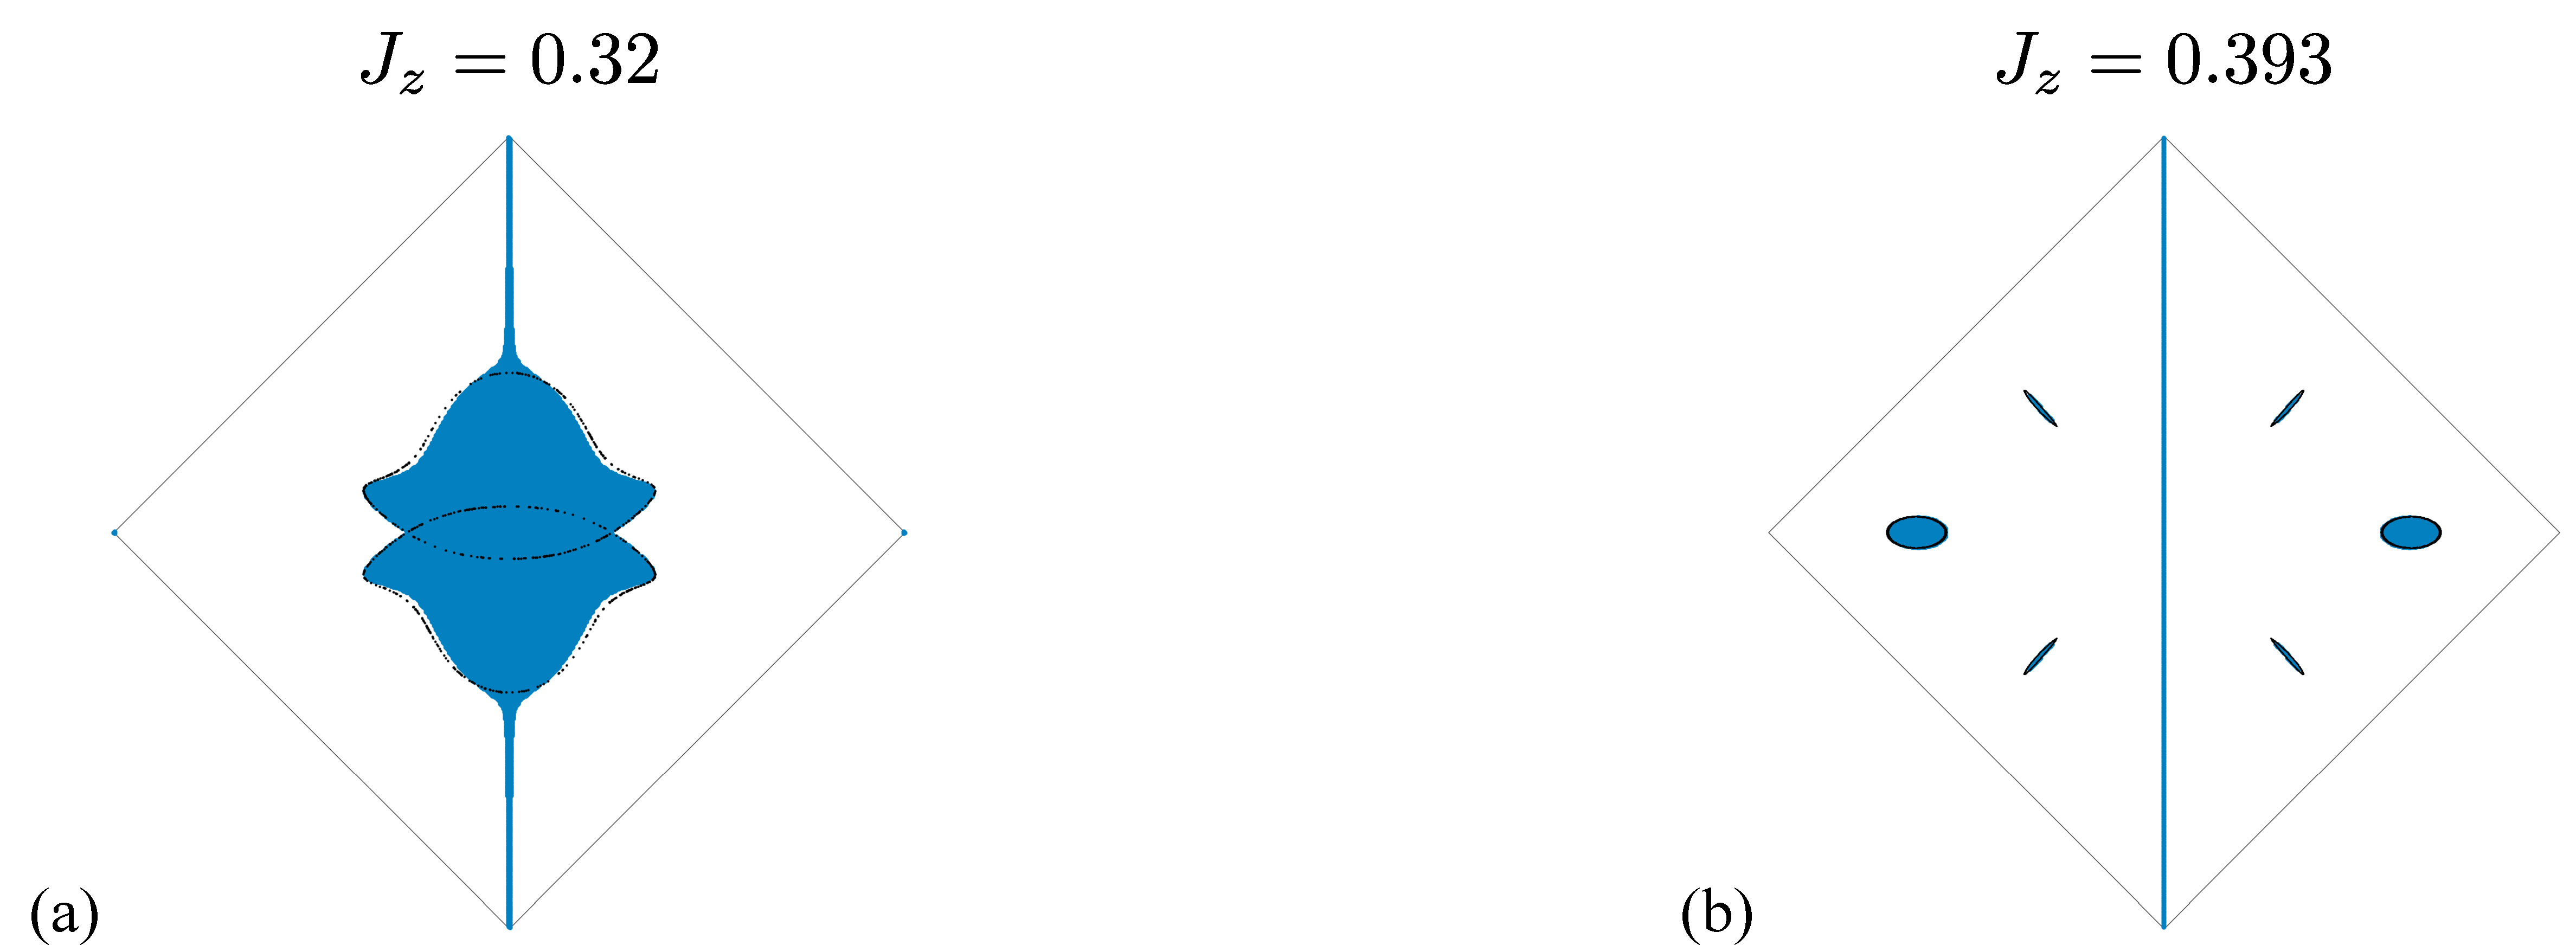
\includegraphics[width=0.8\linewidth]{./chapter06/9_3a_AFIIPanel3.pdf}
	\caption{
		(a) Surface states for $J_z = 0.32$ depicted in blue along with projection of bulk nodal lines depicted in black for the 001-surface Brillouin zone of lattice (9,3)a.
		(b) Surface states for $J_z = 0.393$ depicted in blue along with projection of bulk nodal lines depicted in black for the 001-surface Brillouin zone of lattice (9,3)a.
	}
	\label{fig:chapter06_AFIIPanel3}
\end{figure}
%

For the gapless region corresponding to $J_z \gtrsim 0.392$, a number of nodal lines are stabilized by a one-dimensional \ZZ~winding number.
For $J_z \approx 0.392$, a total of six nodal points appear along high-symmetry lines related to one another by inversion and mirror symmetries or, equivalently, by $C_3$ and inversion symmetries.
The high-symmetry lines themselves correspond to momenta invariant under the combination of mirror and inversion symmetries -- one such line for each of the three mirror planes (see Figure~\ref{fig:chapter06_AFIIPanel2}).
As $J_z$ is increased, the point nodes immediately expand to nodal lines which move through the Brillouin zone and are heavily deformed.
Figure~\ref{fig:chapter06_AFIIPanel2} shows the evolution of the nodal lines for several values of $J_z$.
Due to the severe deformation of the nodal lines which occurs, the figure shows a "top" view from which the deformation is significantly less evident in order to give an overview of their evolution.

From the figure it can already be seen that as $J_z$ is increased slightly, the nodal lines touch before splitting once more to a different total number of nodal lines.
For $J_z \gtrsim 0.42$, there is a transition from the AFII flux phase to the SI flux phase, however, if the analysis is carried out further in the AFII flux configuration, the nodal lines are all seen to combine and shrink to the $\Gamma$-point before gapping out entirely at $J_z \approx 0.45$.
%
\begin{figure}[tb]
	\centering
	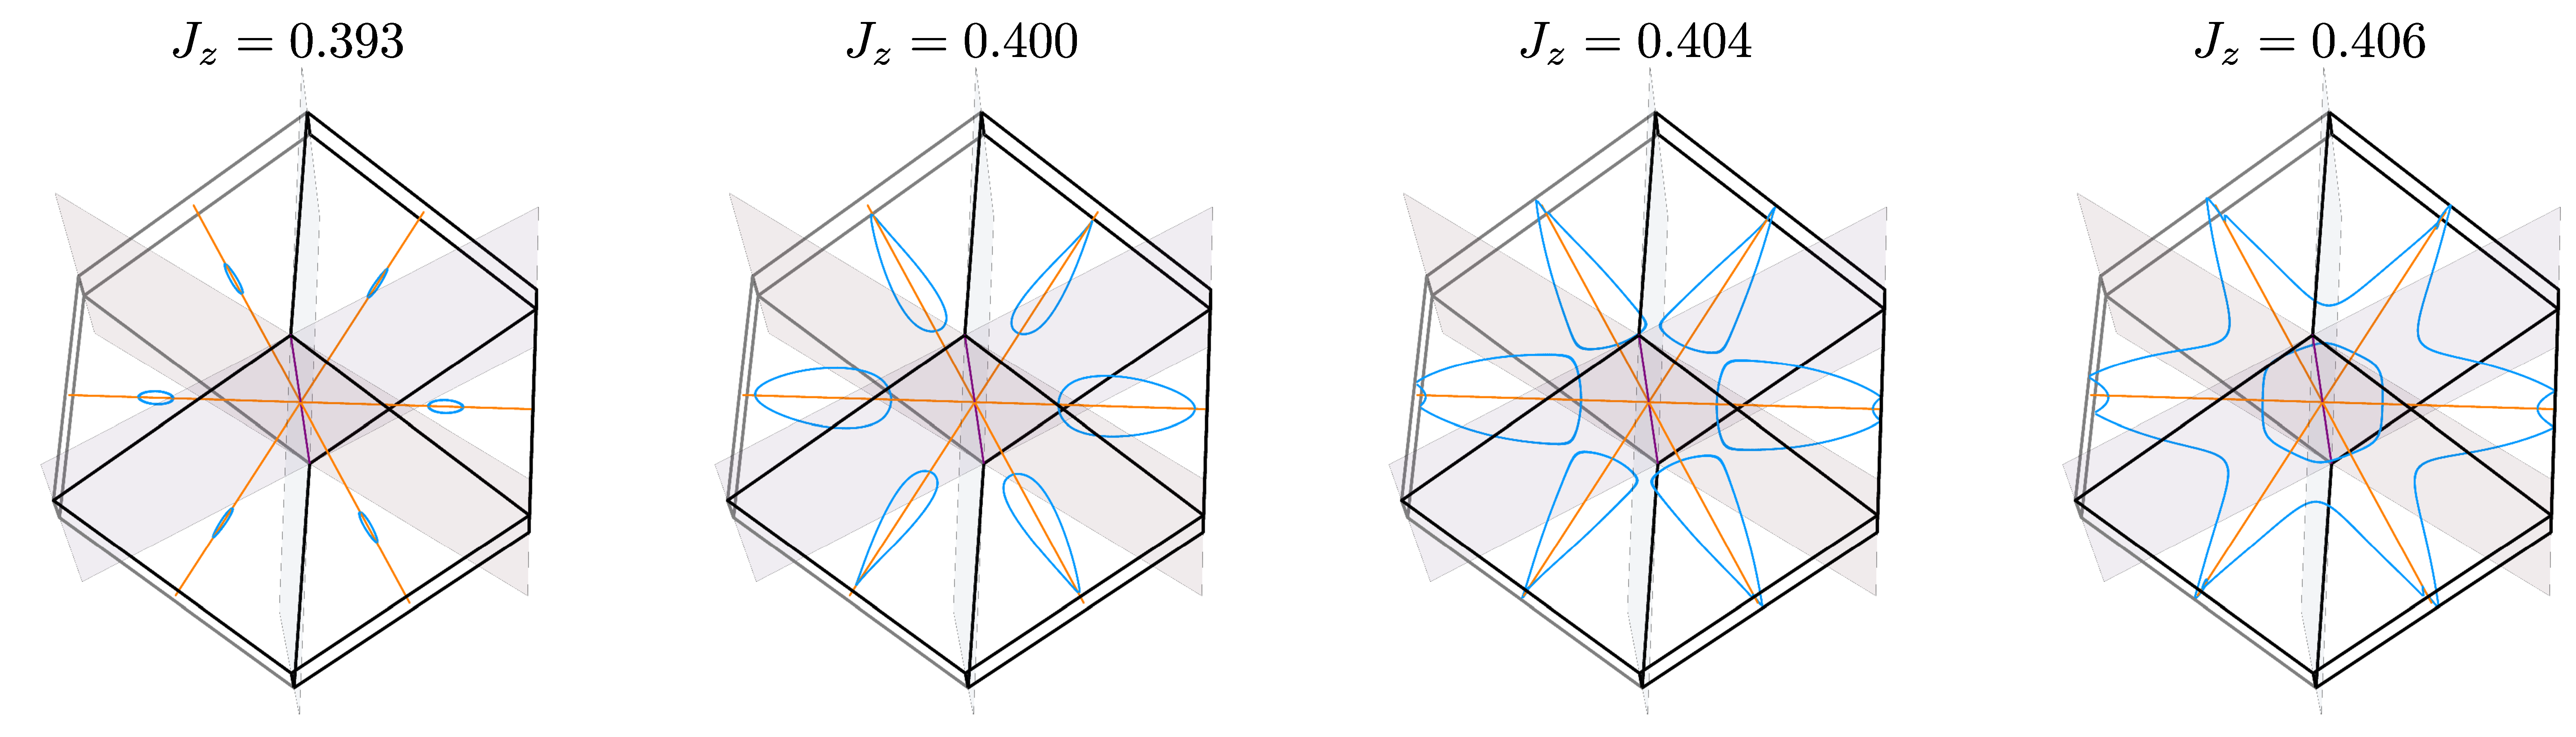
\includegraphics[width=\linewidth]{./chapter06/9_3a_AFIIPanel2.pdf}
	\caption{
		Evolution of nodal lines for several values of $J_z \geq 0.393$ shown in blue.
		The shaded planes denote the three mirror invariant planes, whereas the orange lines denote the $k$-points invariant under a combination of mirror and inversion symmetries.
	}
	\label{fig:chapter06_AFIIPanel2}
\end{figure}
%

Putting the model on a slab geometry (see Figure~\ref{fig:chapter06_AFIIPanel2}~(b)), there are seen to be "drumhead"-type surface states filling the projection of the nodal lines to the surface Brillouin zone as well as the remnant of a Fermi arc from the \ZZ~monopole nodal lines which appear in another part of the phase diagram as discussed above.
However, no Fermi arc like states are observed connecting the disjoint projections of the bulk nodal lines.
The lack of such Fermi arc surface states along with the fact that the bulk nodal lines are not created and destroyed in pairs, rather they appear individually at arbitrary points in the Brillouin zone, indicates that they carry a one-dimensional winding number rather than the two-dimensional monopole charge.


%
%
%%%%%%%%%%%%%%%%%%%%%%%%%%%%%%%%%%%%%%%%%%%%%%%%%%%%%%%%%%%%%%%%%%%%%%%%%%%%%%%%%%%%%%%%
\section{Summary and outlook}
\label{section:chapter06_Conclusion}
%%%%%%%%%%%%%%%%%%%%%%%%%%%%%%%%%%%%%%%%%%%%%%%%%%%%%%%%%%%%%%%%%%%%%%%%%%%%%%%%%%%%%%%%
%
%
This chapter served as a reexamination of the Kitaev model defined on the hypernonagon lattice (9,3)a originally discussed in the work of Reference~\cite{OBrienPRB2016}.
Due to the lattice being non-bipartite, the ground state flux configuration is known to break time-reversal symmetry spontaneously, resulting in a chiral spin liquid ground state.
As mentioned already in Chapter~\ref{chapter:ClassificationOfKSL}, however, the previous analysis of the Kitaev model on this lattice mapped out the fermionic phase diagram using a simple flux configuration which was known not to correspond to the ground state.

In the work reported on in the present chapter, the chiral spin liquids in the entire parameter regime were studied using a combination of finite temperature quantum Monte Carlo simulations, variational calculations and analytic techniques.
The numerics indicate that the phase diagram hosts a variety of chiral spin liquid ground states whose flux sectors depend on the values of the exchange couplings.
A total of five distinct ground state flux configurations were found for different portions of the phase diagram.
While two of these chiral spin liquid ground states are found to be fully gapped, the remaining three ground state flux configurations are seen to correspond to both fully gapped \textit{and} gapless regions in parameter space.

The gapless fermionic excitations in the flux sectors denoted SI and AF are the same Weyl nodes predicted by the classification scheme detailed in Chapter~\ref{chapter:ClassificationOfKSL} which makes use of the projective symmetries of the gauge \textit{Ansatz}.
The analysis of the so-called AFII flux phase, however, sheds light on the possibility of symmetry protected nodal manifolds which were overlooked by the aforementioned classification scheme.
According to this scheme, chiral Kitaev spin liquids cannot host stable nodal lines.
This determination was made based on the inability to define a certain one-dimensional winding number for systems lacking projective time-reversal symmetry~\cite{ZhaoPRL2013,MatsuuraNJP2013}.
However, it has been shown that nodal lines in a three-dimensional system may also be protected by one- or two-dimensional \ZZ~winding numbers in the presence of combined inversion and time-reversal symmetries~\cite{KimPRL2015,FangPRB2015}.
Nodal lines with a \ZZ~monopole charge are seen to exist for a range of exchange couplings in the AFII flux phase.
In yet another parameter regime, this flux phase hosts nodal lines which instead are stabilized by the one-dimensional variant of the \ZZ~winding number.

While much of the results in this chapter are in line with the predictions of the classification scheme detailed in Chapter~\ref{chapter:ClassificationOfKSL}, some results indicate an even richer Kitaev spin liquid physics than previously understood.
The existence of stable monopole nodal lines is possible in principle for any Kitaev spin liquid possessing both inversion and time-reversal symmetries so long as the corresponding projective symmetries are implemented without a finite nesting vector  -- note that this combination of symmetries prevents the formation of stable Weyl nodes.
As seen in this chapter, such nodal lines are also stable for a chiral spin liquid with a broken inversion symmetry, where the combination of time-reversal and inversion operations \textit{does} yield a symmetry.